% !TeX program = xelatex
\documentclass[t, aspectratio=169, 11pt]{beamer}

\usepackage{fontspec}
\setmainfont{Times New Roman}
\setsansfont{Arial}
\setmonofont[Scale=0.9]{Courier New}
\usepackage{amsthm,amsmath,amssymb,mathtools}
\usepackage{bm}
\usepackage{array,booktabs,multirow,makecell}
\usepackage{colortbl}
\usepackage{tikz}
\usepackage[normalem]{ulem}
\usepackage{etoolbox}
\usetikzlibrary{positioning,calc,arrows.meta,backgrounds,shapes.geometric}

\makeatletter
\patchcmd{\beamer@sectionintoc}{\vskip1.5em}{\vskip0.55em}{}{}
\makeatother

% --- CẤU HÌNH LỀ ---
\def\slideContentLeftMargin{0.5cm}
\def\slideContentRightMargin{1cm}
\def\hustHeaderHeight{1cm}
\def\slideContentBotMargin{2.5cm}
\def\slideContentTopPadding{1.3cm}

\usepackage[red, 169]{beamerthemeHUST}

\graphicspath{{images/}{../reports/figures/}{./}}

\setbeamertemplate{footline}{\vspace{2.3cm}}
\setbeamertemplate{itemize item}{\textbullet}
\setbeamertemplate{itemize subitem}{\small\textbullet}
\setbeamertemplate{itemize subsubitem}{\small\textbullet}
\setbeamercolor{itemize item}{fg=black!80}
\setbeamercolor{itemize subitem}{fg=black!70}
\setbeamercolor{itemize subsubitem}{fg=black!70}

\renewcommand{\titlePageTitleX}{-0.5cm}
\renewcommand{\titlePageTitleY}{-0.5cm}
\renewcommand{\hustTitleAlign}{\alignLeft}
\renewcommand{\hustSubtitleAlign}{\alignLeft}
\renewcommand{\hustAuthorAlign}{\alignLeft}
\renewcommand{\hustInstAlign}{\alignLeft}

\title{Hệ hỗ trợ quyết định (DSS) điều phối giao Pizza}
\subtitle{Từ dữ liệu thô, dự báo học máy đến tối ưu vận tải và Dashboard}
\author{\textbf{Nhóm 29}}
\institute{
Đại học Bách khoa Hà Nội -- Khoa Toán Tin \\
Giảng viên: TS. Lê Hải Hà \quad \quad Hướng dẫn TH: TS. Trịnh Đình Thăng
}
\date{Tháng 6 năm 2026}

\begin{document}

\begin{frame}[plain]
    \titlepage
\end{frame}

\begin{frame}{1. Bài toán \& Quyết định cần hỗ trợ}
    \begin{columns}
        \column{0.5\linewidth}
        \textbf{Bài toán thực tế}
        \begin{itemize}
            \item Cửa hàng nhận nhiều đơn cùng lúc. Nguồn lực tài xế có hạn.
            \item Điều phối viên cần biết đơn nào nguy cơ trễ cao để ưu tiên giao trước.
        \end{itemize}
        
        \vspace{0.4cm}
        \textbf{Hệ hỗ trợ quyết định (DSS)}
        \begin{itemize}
            \item \textbf{Input:} Dữ liệu đơn hàng lúc mới đặt.
            \item \textbf{Predictive:} AI dự báo xác suất trễ.
            \item \textbf{Prescriptive:} Gợi ý hành động \& Gán tài xế tối ưu.
        \end{itemize}
        
        \column{0.48\linewidth}
        \centering
        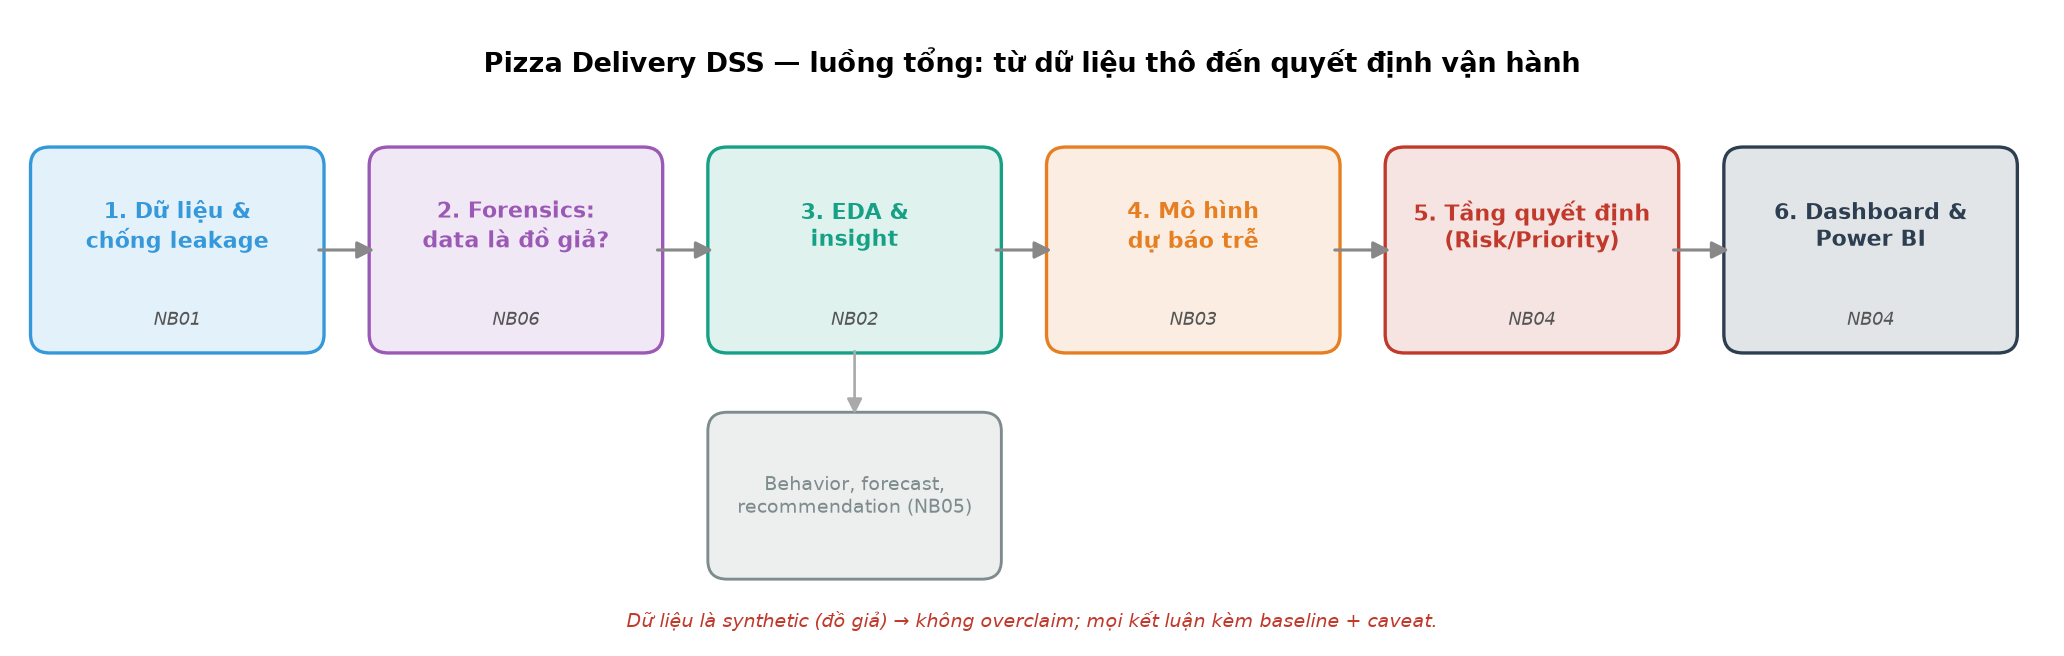
\includegraphics[width=\linewidth,height=0.6\textheight,keepaspectratio]{../reports/figures/pipeline_overview.png}
    \end{columns}
\end{frame}

\begin{frame}{2. Dữ liệu, Rò rỉ (Leakage) \& Ngưỡng mục tiêu}
    \begin{columns}
        \column{0.5\linewidth}
        \textbf{Ngăn chặn Data Leakage:}
        \begin{itemize}
            \item Chỉ dùng dữ liệu có sẵn ngay lúc đặt hàng. Các cột như \texttt{delivery\_duration\_min} bị \textbf{cấm tuyệt đối} để mô hình không "học vẹt".
        \end{itemize}
        
        \vspace{0.4cm}
        \textbf{Xác định ngưỡng Trễ (Delay Threshold):}
        \begin{itemize}
            \item Bằng thuật toán quét (Sweep), ta tìm được luật của dữ liệu: Mọi đơn \texttt{duration $\ge$ 35} đều bị gắn mác Trễ. 
            \item Ngưỡng thực tế là 30 phút.
        \end{itemize}

        \column{0.48\linewidth}
        \centering
        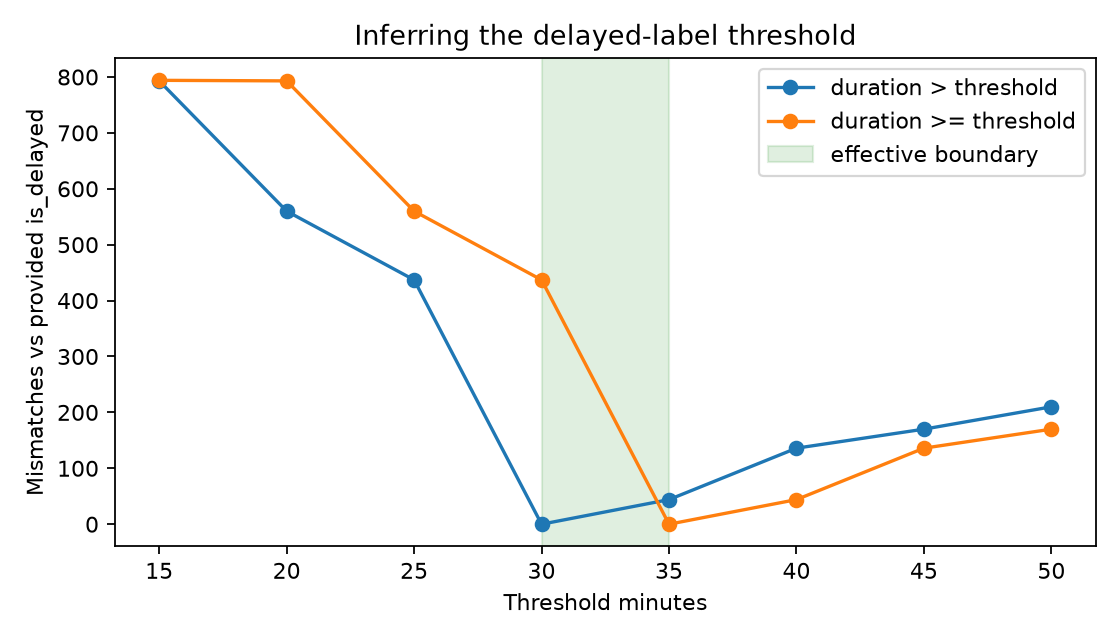
\includegraphics[width=\linewidth,height=0.6\textheight,keepaspectratio]{../reports/figures/delay_threshold_inference.png}
    \end{columns}
\end{frame}

\begin{frame}{3. Khám định Dữ liệu (Synthetic Forensics)}
    \begin{columns}
        \column{0.5\linewidth}
        \textbf{Tại sao phải Khám định?}
        \begin{itemize}
            \item Để chứng minh dữ liệu Kaggle này là dữ liệu sinh tự động (Synthetic) bằng thuật toán.
            \item Đảm bảo nhóm không \textit{overclaim} (nói quá) về độ chính xác kinh doanh thực tế.
        \end{itemize}
        
        \vspace{0.3cm}
        \textbf{Bằng chứng:}
        \begin{itemize}
            \item 4 tính năng (như Estimated Duration, Pizza Complexity) là công thức toán học nội suy 100\% từ cột khác (Sai số = 0).
            \item Quyết định: Loại bỏ chúng khỏi \textbf{Compact Feature Set} để chống đa cộng tuyến.
        \end{itemize}
        
        \column{0.48\linewidth}
        \centering
        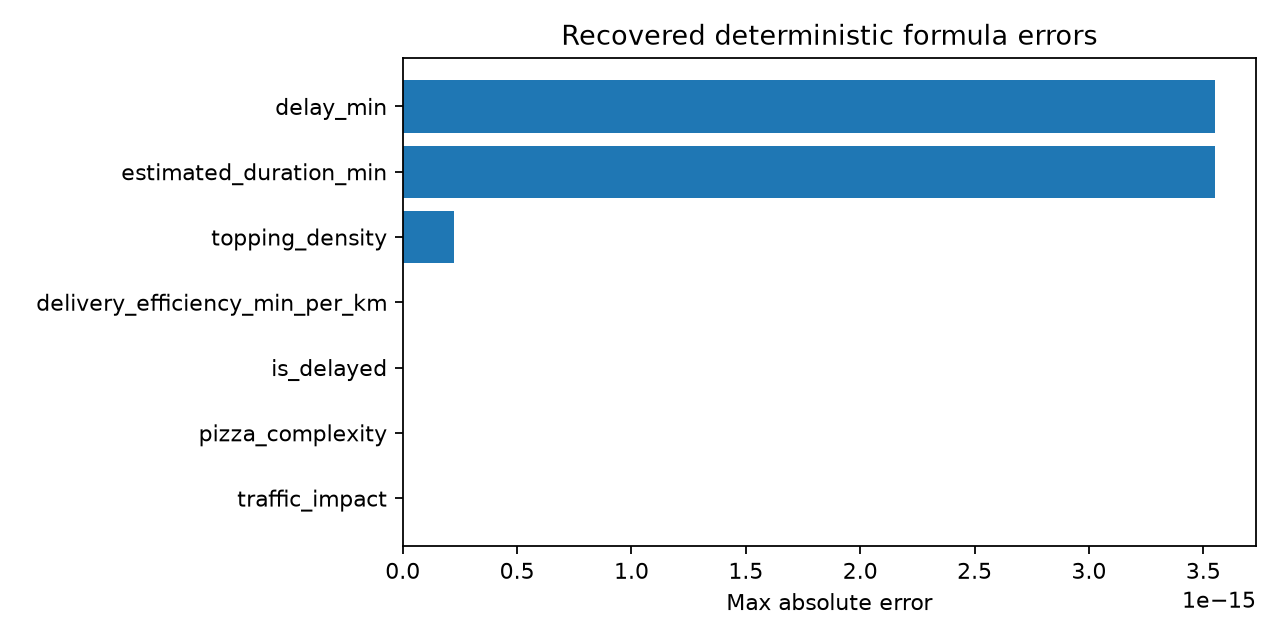
\includegraphics[width=\linewidth,height=0.6\textheight,keepaspectratio]{../reports/figures/generator_deterministic_formula_errors.png}
    \end{columns}
\end{frame}

\begin{frame}{4. Phân tích Khám phá (EDA) Cốt lõi}
    \begin{columns}
        \column{0.48\linewidth}
        \textbf{Mất cân bằng nhãn (Imbalance)}
        \begin{itemize}
            \item Chỉ có $\sim 21\%$ đơn là trễ. 
            \item Không thể dùng Accuracy để đánh giá (Đoán "Luôn đúng giờ" cũng đạt 79\%).
        \end{itemize}
        \vspace{0.4cm}
        \textbf{Driver gây trễ (Traffic \& Distance)}
        \begin{itemize}
            \item Mức kẹt xe (High Traffic) làm tỷ lệ trễ vọt lên rất cao. Đây là insight vận hành mấu chốt để lập quy tắc phạt.
        \end{itemize}

        \column{0.5\linewidth}
        \centering
        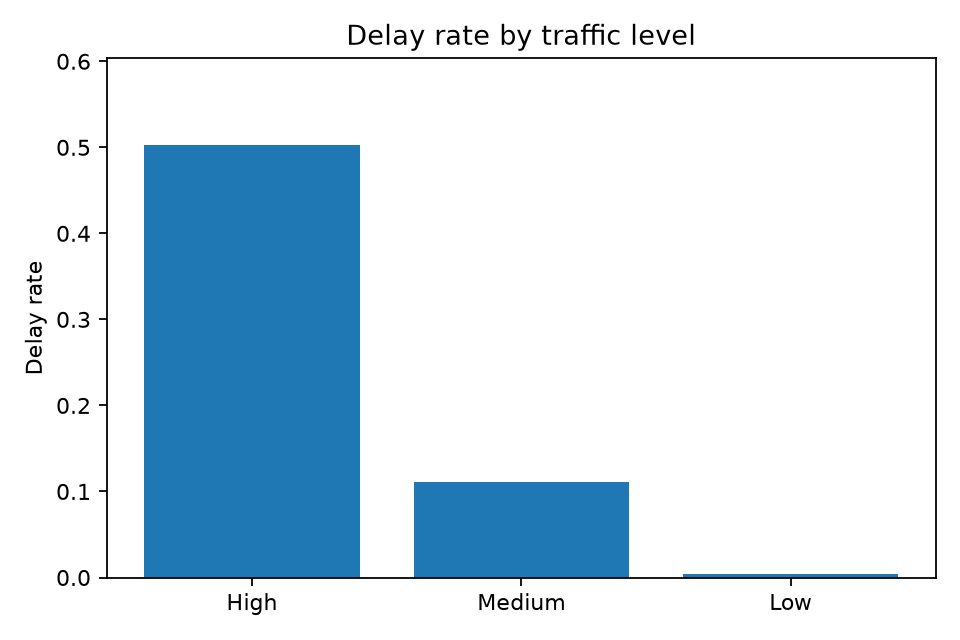
\includegraphics[width=\linewidth,height=0.6\textheight,keepaspectratio]{../reports/figures/delay_rate_by_traffic.png}
    \end{columns}
\end{frame}

\begin{frame}{5. So sánh Mô hình \& Tại sao không chọn Bayes?}
    \begin{columns}
        \column{0.5\linewidth}
        \textbf{Kiểm thử 6 họ mô hình (Classifiers):}
        \begin{itemize}
            \item \textbf{Logistic Regression (LR):} Chiến thắng với F2 tốt nhất (0.943), ít Overfit, dễ diễn giải.
            \item \textbf{SVM \& Random Forest:} Bám sát nhưng chậm và phức tạp hơn.
            \item \textbf{Tại sao loại Naive Bayes?} Điểm F2 cực thấp (0.66). Lý do: Thuật toán này giả định các tính năng độc lập, trong khi dữ liệu giao hàng có tính liên kết chặt chẽ.
        \end{itemize}
        
        \column{0.48\linewidth}
        \centering
        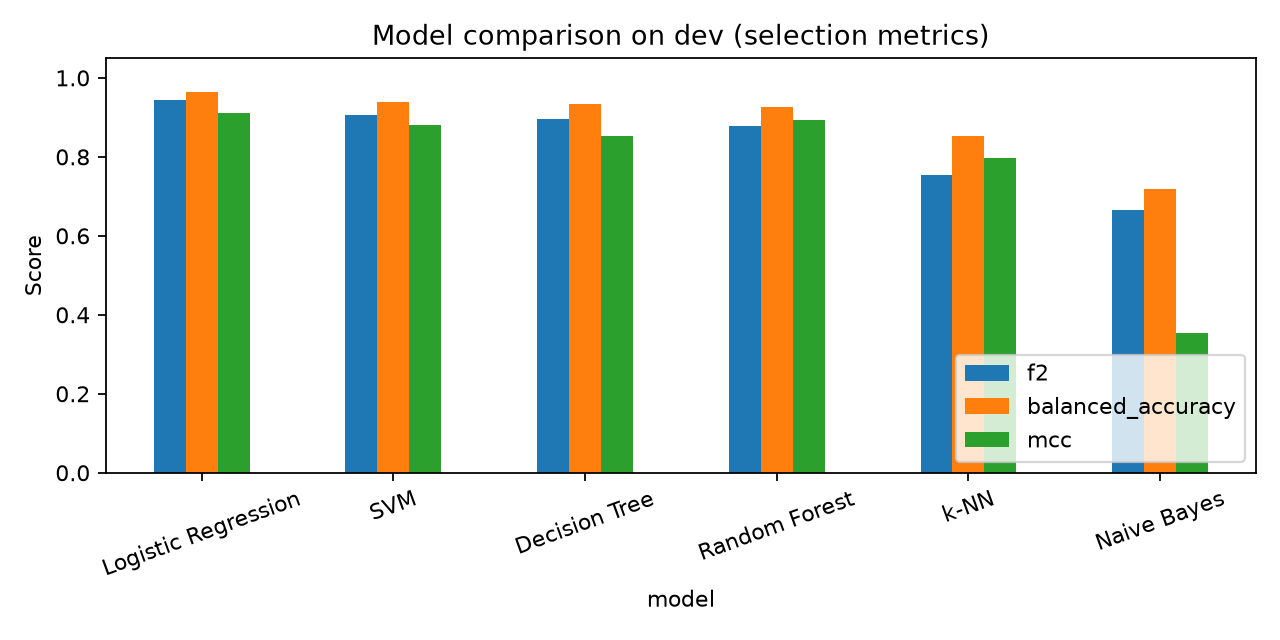
\includegraphics[width=\linewidth,height=0.6\textheight,keepaspectratio]{../reports/figures/model_comparison.png}
    \end{columns}
\end{frame}

\begin{frame}{6. F-Beta, Tuning \& Độ Ổn định}
    \begin{columns}
        \column{0.48\linewidth}
        \textbf{Tuning \& Metric}
        \begin{itemize}
            \item \textbf{Ưu tiên F2-Score:} Việc bỏ sót đơn trễ (False Negative) đắt giá hơn nhiều so với việc cảnh báo thừa (False Positive).
            \item \textbf{Tuning Logistic Reg:} Giữ nguyên $C=1.0$ do dữ liệu synthetic phân cực sẵn, tune tiếp không đem lại lợi ích rõ rệt.
        \end{itemize}
        
        \column{0.5\linewidth}
        \textbf{Độ Ổn định (Stability Audit)}
        \begin{itemize}
            \item Chạy \textit{100 lần chia Random Split} (Train/Dev).
            \item Điểm F2 không dao động nhiều. Kết quả xuất sắc không phải do "ăn may".
        \end{itemize}
        \vspace{0.2cm}
        \centering
        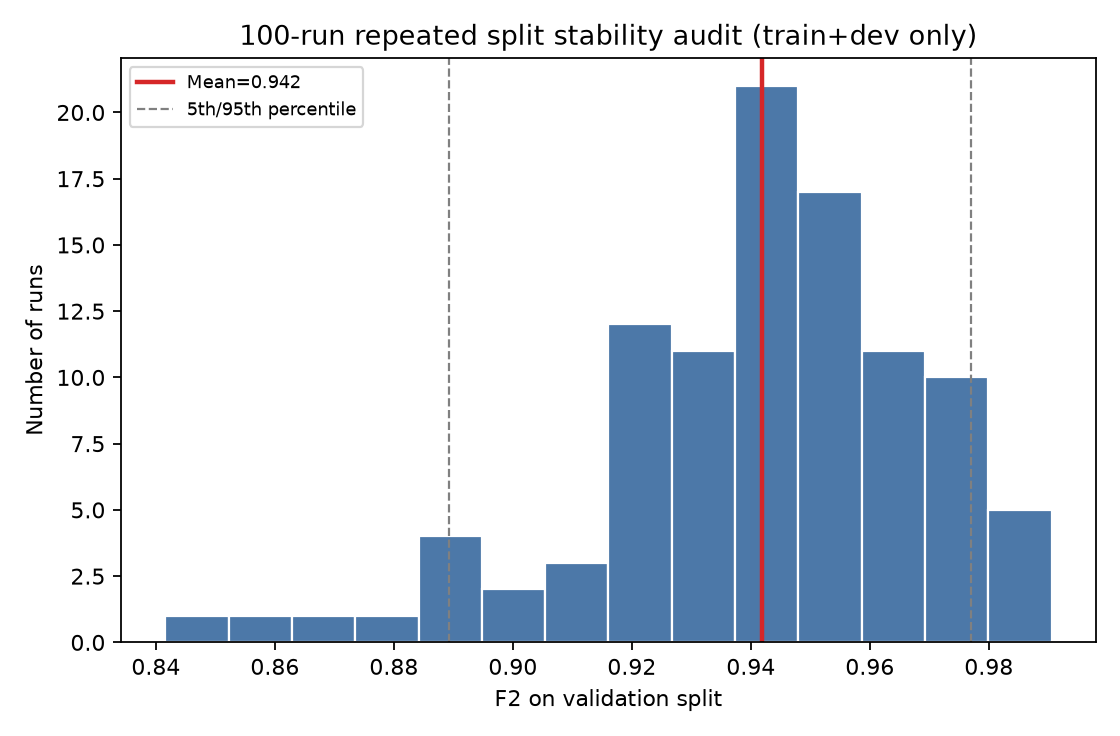
\includegraphics[width=0.8\linewidth,height=0.3\textheight,keepaspectratio]{../reports/figures/model_stability_f2_distribution.png}
    \end{columns}
\end{frame}

\begin{frame}{7. Kết quả Test sau khi Khóa mô hình}
    \begin{columns}
        \column{0.45\linewidth}
        \textbf{Đánh giá Test-set}
        \begin{table}
            \centering
            \begin{tabular}{lr}
            \toprule
            Metric & Giá trị\\
            \midrule
            Accuracy & 0.960\\
            \textbf{Balanced Acc} & \textbf{0.966}\\
            Precision & 0.854\\
            \textbf{Recall} & \textbf{0.976}\\
            \textbf{F2-Score} & \textbf{0.949}\\
            MCC & 0.889\\
            \bottomrule
            \end{tabular}
        \end{table}
        
        \column{0.52\linewidth}
        \textbf{So sánh Baseline}
        \begin{itemize}
            \item \textbf{Always On-time:} F2 = 0.
            \item \textbf{Always Delayed:} F2 = 0.569.
            \item Logistic Regression (F2 = 0.949) hoàn toàn vượt trội Baseline.
            \item \textbf{Kết luận:} Recall 97.6\% có nghĩa là mô hình gần như \textbf{không bỏ lọt} bất kỳ đơn nào bị trễ.
        \end{itemize}
    \end{columns}
\end{frame}

\begin{frame}{8. Xây dựng Trọng số Rủi ro (Risk Score)}
    \begin{columns}
        \column{0.5\linewidth}
        \textbf{Từ Mô hình đến Nghiệp vụ}
        \begin{itemize}
            \item AI không làm "Black Box".
            \item \textbf{Delay Risk Score (0-100)} = (0.55 $\times$ Xác suất AI) + (0.45 $\times$ Penalty Vận hành: Giao thông, Khoảng cách...).
            \item Điều phối viên nhìn vào đơn hàng sẽ biết ngay vì sao điểm rủi ro lại cao.
        \end{itemize}
        
        \column{0.48\linewidth}
        \centering
        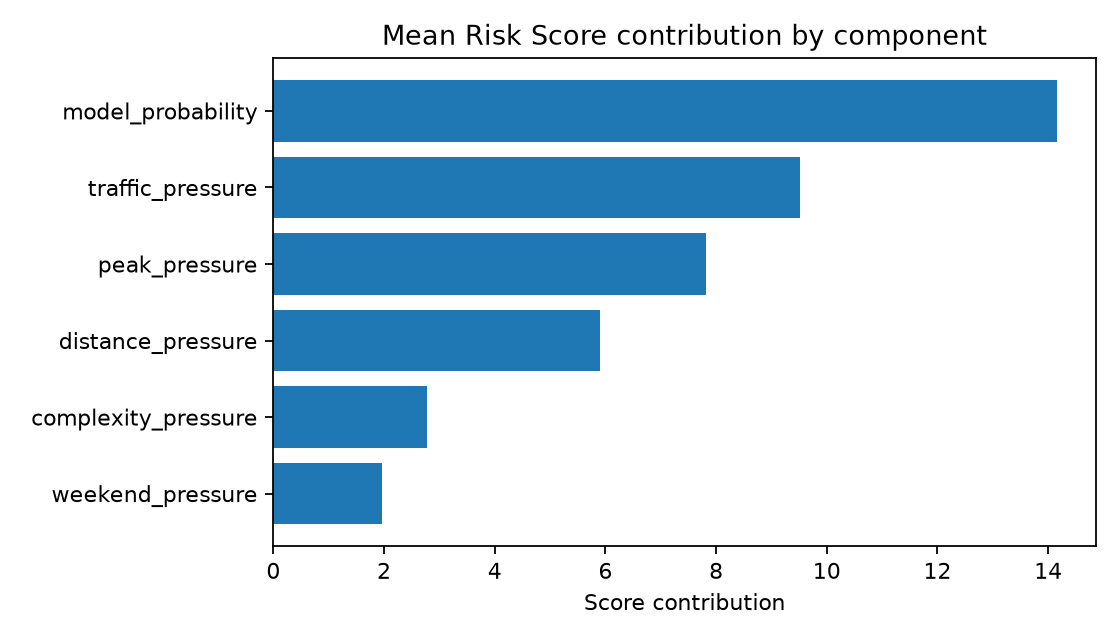
\includegraphics[width=\linewidth,height=0.6\textheight,keepaspectratio]{../reports/figures/risk_component_breakdown.png}
    \end{columns}
\end{frame}

\begin{frame}{9. Delay Priority Queue \& Gợi ý Hành động}
    \begin{columns}
        \column{0.55\linewidth}
        \textbf{Hàng đợi \& Phân luồng ưu tiên}
        \begin{itemize}
            \item \textbf{High (> 65):} Khuyến nghị gán tài xế ưu tiên, báo khách hàng nguy cơ trễ.
            \item \textbf{Medium (35 - 65):} Đẩy nhanh tiến độ làm bánh.
            \item \textbf{Low (< 35):} Xử lý bình thường.
        \end{itemize}
        
        \column{0.4\linewidth}
        \begin{center}
            Hệ thống liên tục quét đơn mới để đẩy lên đỉnh \textbf{Priority Queue}, giúp cửa hàng đối phó với giờ cao điểm (Peak Hours).
        \end{center}
    \end{columns}
\end{frame}

\begin{frame}{10. Ứng dụng Thực tế: Streamlit Dashboard}
    \begin{itemize}
        \item Cung cấp hệ thống tương tác \textbf{Web-based} cho Quản lý / Điều phối viên.
        \item \textbf{8 Phân hệ tích hợp:} Báo cáo tổng quan, EDA, Forecasting, Model Eval và Action Queue.
        \item Cung cấp tính năng \textbf{Single Order Demo}: Nhập dữ liệu 1 đơn $\Rightarrow$ Nhận Risk Score \& Explainable breakdown tức thì.
    \end{itemize}
    \vspace{0.8cm}
    \begin{center}
        \textit{(Trình chiếu Dashboard trực tiếp)}
    \end{center}
\end{frame}

\begin{frame}{11. Bài toán Tối ưu Vận tải (Transportation Problem)}
    \begin{columns}
        \column{0.48\linewidth}
        \textbf{Minh họa Prescriptive DSS}
        \begin{itemize}
            \item Lấy các đơn hàng \textbf{High Priority}. Giả lập mạng lưới tài xế.
            \item \textbf{Cost Matrix:} Phạt nặng nếu đơn rủi ro mà không có tài xế, thưởng nếu giao cùng tuyến.
            \item \textbf{Thuật toán:} Tối ưu hóa toàn cục chi phí giao hàng bằng thuật toán \textbf{Hungarian}.
        \end{itemize}
        
        \column{0.5\linewidth}
        \centering
        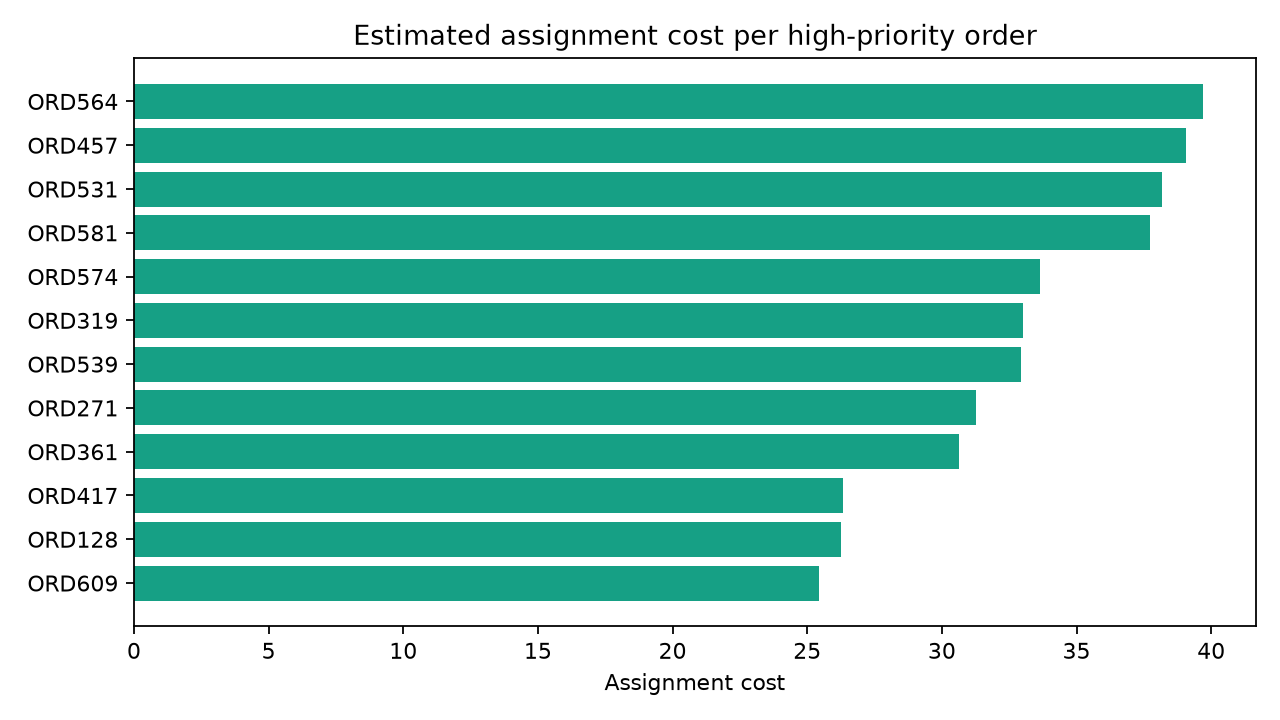
\includegraphics[width=\linewidth,height=0.6\textheight,keepaspectratio]{../reports/figures/transport_assignment_cost.png}
    \end{columns}
\end{frame}

\begin{frame}{12. Giới hạn \& Kết luận}
    \begin{columns}
        \column{0.48\linewidth}
        \textbf{Hạn chế (Caveats)}
        \begin{itemize}
            \item \textbf{Dữ liệu sinh (Synthetic):} Forecast nhu cầu hay Preference trends không mang ý nghĩa thị trường thực, chỉ mang tính minh họa phương pháp luận.
            \item Tài xế trong bài toán vận tải chỉ là tham số giả lập.
        \end{itemize}
        
        \column{0.48\linewidth}
        \textbf{Kết luận}
        \begin{itemize}
            \item Hoàn thiện một chu trình \textbf{DSS khép kín}.
            \item Đảm bảo độ nghiêm ngặt khoa học (ngăn rò rỉ, giải thích được).
            \item Sẵn sàng triển khai thành công cụ vận hành.
        \end{itemize}
    \end{columns}
\end{frame}

\end{document}
